% A local step resets at the exact state; global error propagates the computed path.
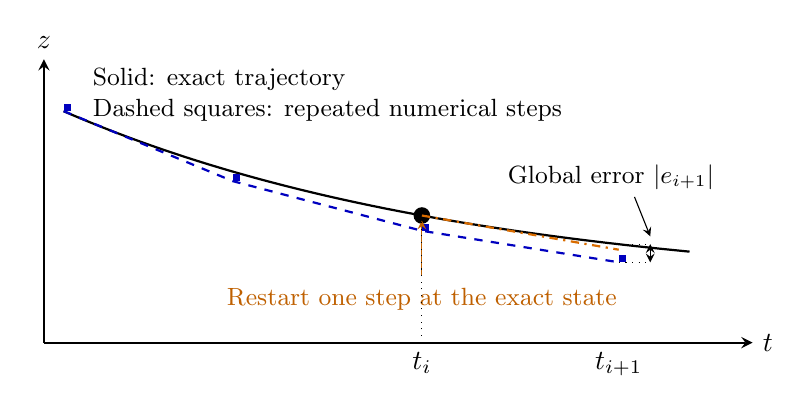
\begin{tikzpicture}[>=stealth,font=\normalsize]
\draw[->,thick](0,0)--(9,0)node[right]{$t$};\draw[->,thick](0,0)--(0,3.6)node[above]{$z$};
\draw[black,thick,domain=.25:8.2,samples=70]plot(\x,{.65+2.4*exp(-.19*\x)});
\draw[blue!75!black,thick,dashed](.25,2.94)--(2.4,2.05)--(4.8,1.42)--(7.3,1.02);
\foreach \x/\y in {.25/2.94,2.4/2.05,4.8/1.42,7.3/1.02}{\fill[blue!75!black](\x,\y)rectangle+(0.09,0.09);}
\fill(4.8,1.614)circle(3pt);\draw[orange!85!black,thick,dash dot](4.8,1.614)--(7.3,1.18);
\draw[dotted](7.3,1.02)--(7.7,1.02);\draw[dotted](7.3,1.25)--(7.7,1.25);
\draw[<->](7.7,1.02)--(7.7,1.25);
\node[font=\small]at(7.2,2.1){Global error $|e_{i+1}|$};
\draw[->](7.5,1.85)--(7.7,1.35);
\node[align=left,font=\small]at(3.6,3.15){Solid: exact trajectory\\Dashed squares: repeated numerical steps};
\node[align=center,font=\small,orange!75!black]at(4.8,.55){Restart one step at the exact state};
\draw[->,orange!75!black](4.8,.85)--(4.8,1.55);
\draw[dotted](4.8,0)--(4.8,1.55);\node[below]at(4.8,0){$t_i$};\node[below]at(7.3,0){$t_{i+1}$};
\end{tikzpicture}
